
\section{Intelligenza Artificiale}
L'Intelligenza Artificiale è la scienza che si occupa di creare sistemi informatici 
in grado di svolgere compiti che normalmente richiedono l’intelligenza umana, 
come il riconoscimento di oggetti, la comprensione del linguaggio naturale, la 
risoluzione di problemi e l’apprendimento.
In altre parole, l’IA è un ramo dell’informatica che studia la progettazione di 
agenti intelligenti.
% , ovvero sistemi capaci di percepire l’ambiente in cui 
% operano e di agire perseguendo specifici scopi.
L’IA, pertanto, è la capacità delle macchine di simulare le capacità 
cognitive umane, come il ragionamento e la pianificazione \cite{IA_1,IA_EM_SH, IA_ML_DL}.

% Questa disciplina è un ambito molto dibattuto sia tra scienziati che tra filosofi, 
% in quanto manifesta aspetti etici, oltre che teorici e pratici. 
% Le grandi menti mondiali hanno menzionato a più
% riprese, nei loro interventi, i pericoli di un’intelligenza artificiale mal gestita:
% Stephen Hawking, nel 2014, la considerò una minaccia per la sopravvivenza
% umana; Elon Musk, nello stesso anno, la definì più pericolosa del nucleare.
% Tuttavia, i vantaggi di un utilizzo consapevole dell’intelligenza artificiale come
% ambito di sviluppo e di progresso sembrano aver superato i rischi, tant'è che al
% giorno d’oggi è diventata parte del quotidiano \cite{IA_EM_SH, IA_1}.

Come si può osservare dalla figura (\ref{fig:rappresentazione dell'IA, ML e DL}), 
il campo dell'intelligenza artificiale è un'area di studio che include molteplici 
discipline.

\begin{figure}[H]
    \centering
    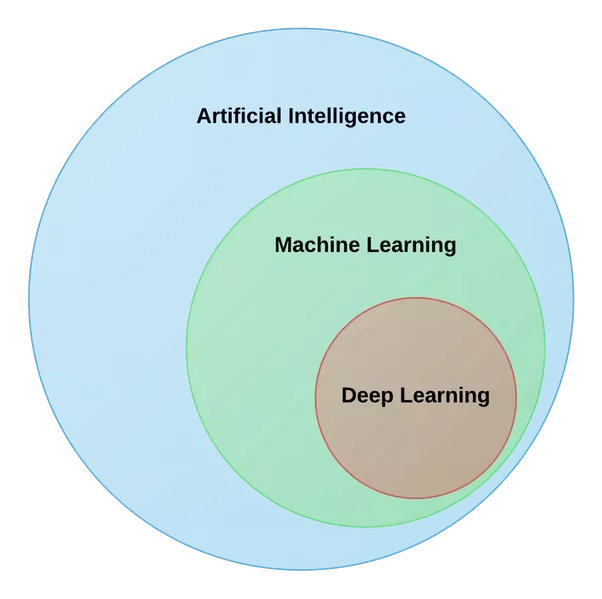
\includegraphics[width=0.44\textwidth]{Immagini/Generiche/AI_ML_DL_Differenze_v2.png}
    \caption{Rappresentazione delle categorie \cite{INGLOBAZIONE_IA}.} 
    \label{fig:rappresentazione dell'IA, ML e DL}
    %Figura 2.1: Esempio schematico di un neurone
\end{figure}
Ciascuna di queste discipline può essere vista come un elemento del livello precedente.
Il Machine Learning rappresenta un sottoinsieme dell’Intelligenza Artificiale. 
Il Deep Learning, a sua volta, è un sottoinsieme del Machine Learning e le 
reti neurali costituiscono l'elemento fondamentale degli 
algoritmi di Deep Learning.
Si può anche dire che l'Intelligenza Artificiale è la disciplina di base e il Machine 
Learning e il Deep Learning le tecniche che ne consentono 
l’applicazione \cite{IA_1,IA_ML_DL}. 


% \subsection{Cenni storici}
% Si può dire che l’AI nasce con l’avvento dei computer, nella seconda metà
% degli anni cinquanta. Il primo programma di un sistema intelligente riguardava solo la
% dimostrazione di alcuni teoremi matematici partendo da determinate informazioni. 
% Successivamente, molte università e aziende americane come l’IBM si
% cimentarono nello sviluppo di programmi e software in grado di pensare come
% gli esseri umani.
% Col passare degli anni vennero sviluppati software sempre più complicati
% dal punto di vista matematico ma, contrariamente a quello che si sperava,
% l’intelligenza artificiale sembrava non riuscire a riprodurre le caratteristiche
% intellettuali umane. Il progresso definitivo si ebbe con l’avvento delle reti
% neurali, che hanno permesso ai sistemi intelligenti di migliorare sempre di più
% le proprie capacità di comportamento. Ora, questi sistemi sono in grado di
% prendere decisioni senza l’intervento umano ed effettuare scelte a seconda del
% contesto in cui sono inseriti \cite{IA_1}.


\section{Machine Learning}
\subsection{Definizione}

Machine Learning comprende un insieme di metodi con cui si allena l’intelligenza artificiale 
a svolgere delle attività non programmate, a imparare dall’esperienza passata, 
come fa esattamente l’intelligenza umana, correggendosi 
e quindi migliorandosi attraverso gli errori commessi.
Questa disciplina viene chiamata anche apprendimento automatico, poiché il modello
impara dalla propria esperienza, senza la necessità di inserire 
nuove istruzioni \cite{IA_ML_DL}.

% Per fare ciò vengono usati algoritmi di regressione o di classificazione 
% per comprendere i dati a disposizione. 

\subsection{Le modalità dell’apprendimento}
Gli algoritmi di apprendimento automatico possono essere suddivisi i quattro categorie 
\cite{I_3_PROBLEMI_ML_e_APPRENDIMENTO, ASPETTI_ML}:
\begin{itemize}
    \item \textbf{Apprendimento supervisionato}: vengono presentati al modello una
    serie di esempi ideali costituiti dalla coppia input-output, in modo che
    riesca a capire la correlazione tra le entrate e le uscite.

    \item \textbf{Apprendimento non supervisionato}: al contrario dell’apprendimento
    precedente il modello riceve solo gli input. Deve capire da solo l’output
    da generare senza potersi confrontare con gli esempi dati.

    \item \textbf{Apprendimento per rinforzo}: Al programma viene fornito 
    un feedback per ogni azione che svolge. Un feedback positivo
    che si tradurrà in una ricompensa indica un’azione svolta correttamente,
    al contrario una punizione indicherà un’azione sbagliata.
    
    \item \textbf{Apprendimento semi-supervisionato}: vengono fornite informazioni
    incomplete sotto forma di esempi come nell’apprendimento supervisionato
    e il modello cercherà di prevedere anche quali sono i risultati mancanti.
\end{itemize}

\newpage
\subsection{Tipologie di problemi}
Nel Machine Learning, si possono distinguere tre tipologie di problemi
\cite{I_3_PROBLEMI_ML_e_APPRENDIMENTO, ASPETTI_ML}:

\begin{itemize}
    \item La \textbf{classificazione}, nella quale gli input sono divisi 
    in due o più classi e
    il sistema di apprendimento deve produrre un modello in grado di
    assegnare ad un input una o più classi tra quelle disponibili. Questi tipi
    di task sono tipicamente affrontati mediante tecniche di apprendimento
    supervisionato. Un esempio di classificazione è l’assegnamento di una
    o più etichette ad una immagine in base agli oggetti o soggetti contenuti
    in essa;
    
    \item La \textbf{regressione}, concettualmente simile alla classificazione con la
    differenza che l’output ha un dominio continuo e non discreto.
    Anch'essa è tipicamente affrontata con l’apprendimento supervisionato.

    \item Il \textbf{clustering}, nel quale, come nella classificazione, un insieme di dati
    viene diviso in gruppi che però, a differenza di questa, non sono noti a
    priori. La natura stessa dei problemi appartenenti a questa categoria li
    rende tipicamente dei task di apprendimento non supervisionato.
\end{itemize}


\section{Deep Learning}
\subsection{Definizione}
Il Deep Learning è un sottoinsieme del Machine Learning che si occupa
di analizzare i dati in maniera profonda, solitamente attraverso una rete di
apprendimento che prende decisioni e giunge a conclusioni in base ai dati forniti.
Questo metodo è particolarmente adatto a grandi set di dati, in quanto molto
più preciso, anche se molto più dispendioso in termini di risorse computazionali
e temporali rispetto all’apprendimento automatico.
% Il modello classico del Deep Learning è caratterizzato da gerarchie di
% caratteristiche comuni che mira ad andare in profondità nell’albero gerarchico
% tra i vari strati (per questo motivo viene detto "apprendimento profondo").
Tra i modelli di apprendimento automatico, trovano larga applicazione le reti 
neurali \cite{IA_ML_DL, ASPETTI_DEEP_LEARNING, ASPETTI_DEEP_LEARNING_2}.
% profonde, la convoluzione di reti neurali profonde e le reti neurali ricorsive, le
% quali vengono applicate nella visione artificiale, nel riconoscimento automatico
% del discorso, nell’elaborazione del linguaggio naturale, nel riconoscimento audio
% e nella bioinformatica 
% \cite{IA_ML_DL, ASPETTI_DEEP_LEARNING, ASPETTI_DEEP_LEARNING_2}.